\documentclass[a4paper,10pt]{article}
\usepackage[portuguese]{babel}
\usepackage[utf8x]{inputenc}
\usepackage[T1]{fontenc}
\usepackage{newtxtext,newtxmath} %TimesNewRoman
\usepackage[sectionbib, numbers, comma, sort]{natbib}
\usepackage{chapterbib}
\usepackage[a4paper,top=3cm,bottom=2cm,left=3cm,right=3cm,marginparwidth=2cm]{geometry}
\usepackage{amsmath}
\usepackage{natbib}
\usepackage{graphicx}
\usepackage[svgnames]{xcolor}
\usepackage[colorinlistoftodos]{todonotes}
\usepackage[colorlinks=true, allcolors=ipbbrown]{hyperref}
\usepackage{minted}
\usepackage{adjustbox}

% school colours
\definecolor{ipbgreen}{RGB}{166,204,59}
\definecolor{ipbbrown}{RGB}{153,80,42}

% code block style
\usemintedstyle{arduino}

\title{
\includegraphics[scale=0.5]{ipbeja_logo.png}\\[0.5cm]Sistema de apoio à promoção do turismo rural\\Fase de Webscraping} % Doc name
\author{Gonçalo Amaro -- 17440,\\ Pedro Tomás -- 18962,\\ Vítor Abreu -- 18966} % Doc's author/s
\date{15 de Dezembro, 2021} % Doc date

\def\blankpage{%
      \clearpage%
      \thispagestyle{empty}%
      \addtocounter{page}{-1}%
      \null%
      \clearpage}

\begin{document}
\bibliographystyle{IEEEtranN}

\maketitle

\blankpage{}

{
  \hypersetup{linkcolor=black}
  \tableofcontents
}

\newpage

{
  \hypersetup{linkcolor=black}
  \listoffigures
  \listoftables
}

\newpage

\section{Introdução}

O objectivo desta fase de trabalho é a recolha da informação que será utilizada no decorrer do projecto, isto é, o ``web-scrapping''.

Simplificando, o processo de ``web-scrapping'' é simplesmente a recolha de dados de uma forma automatizada, no nosso caso foi utilizado a linguagem Python juntamente com algumas bibliotecas como a ``BeautifulSoup4''.

Todas as informações recolhidas foram apenas dentro da localidade de Beja e entre todos os resultados alguns até podem ser comuns, umas vez que todos nós recolhemos por exemplo as ``reviews'' dos hotéis, atracções e restaurantes.

\section{Planeamento}

\subsection{Divisão de Tarefas}

Para a realização desta fase de trabalho o grupo decidiu dividir as tarefas e organizá-las a partir da plataforma ``Trello'' (https://trello.com/b/PIApdmTA/pi-2021-22), uma plataforma de gestão de projecto estilo \textit{board} do qual podemos aplicar Kanban, Scrum ou outra AGILE \textit{management framework}.

A divisão de tarefas decidida foi a distribuição de cada um dos três ``websites'' por cada um dos elementos do grupo, pela ordem de dificuldade em congruência linear com o tempo extra-curricular disponível de cada elemento.

Assim sendo, o site ``TripAdvisor'' foi realizado pelo aluno Gonçalo Amaro, o ``Booking'' pelo Pedro Tomás e o ``Zomato'' pelo Vítor Abreu. No final verificou-se que todos conseguiram aceder aos seus devidos ``websites'' e adquirir as informações possíveis via \textit{scraping}.

\subsection{Tecnologias Usadas}

Na realização do \textit{web-scrapping} foi desenvolvido um ambiente virtual de Python 3 para realizar os \textit{scripts} que iriam recolher as informações.

Como forma de organizar todos os pacotes e possíveis actualizações de bibliotecas dentro do código também foi gerado um ficheiro \text{.txt} denominado ``requirements'' que actualizávamos e usávamos sempre que um dos elementos do grupo iria realizar o seu trabalho.

A linguagem optada para a construção dos \textit{scripts} foi o Python já que é uma das mais acessíveis linguagens de programação disponíveis devido à sua simples \textit{syntax} e também pela vasta quantidade de bibliotecas disponibilizadas, das quais temos uma dúzia que são bastante úteis para a realização deste projecto.

Para finalizar, todos os ficheiros foram guardados em formato \text{.csv} uma vez que, como explicado no relatório de progresso anterior, é um formato que é aceite e nos facilita a manipulação de dados (ETL), a alimentação dos dados ao algoritmo de \textit{machine learning}, e pode ser usado com ferramentas de analise de dos e geradores de tabelas (como o PowerBI).

\subsubsection{Ambientes Virtuais de Python}

Neste projecto usamos Ambientes Virtuais de Python. Um ambiente virtual é uma forma de ter várias instâncias paralelas do interpretador de Python, cada uma com diferentes conjuntos de pacotes e diferentes configurações.

Cada ambiente virtual contém uma cópia discreta do interpretador de Python, incluindo cópias dos seus utilitários de suporte como o \href{https://pypi.org/project/pip/}{pip}. Estes contêm também uma zona para instalação de pacotes/bibliotecas localmente (dentro do ambiente virtual), sendo esta a razão principal pela qual foi decido usá-los.

Tendo introduzido a razão, consegue-se perceber o óbvio: sendo este um trabalho de grupo e que posteriormente poderá ser testado pelos docentes ou futuros alunos, ao usar ambientes virtuais podemos fazer ``pip freeze'' para um ficheiro de texto do qual facilita a portabilidade e transmissão de requerimentos do projecto.

Para a criação destes ambientes virtuais foi instalado o \href{https://pypi.org/project/virtualenvwrapper/}{virtualenvwrapper} o qual traz o \href{https://pypi.org/project/virtualenv/}{virtualenv} como dependência e um \textit{set} de extensões para o mesmo, tal como sempre recomendado pelo Professor José Jasnau Caeiro, todos os anos na disciplina de Linguagens de Programação.

\subsubsection{Bibliotecas de Python usadas}

Como dito previamente, na explicação pelo qual o uso de Python, foi referida a grande quantidade de bibliotecas que nos são facilmente fornecidas pelo \href{https://pypi.org/project/pip/}{pip}.

Dentro deste repositório existe (perto de) uma dúzia de bibliotecas que nos permitem facilmente completar as nossas tarefas deste projecto. Dessa dúzia, para esta etapa, foram usadas:

\begin{itemize}
  \item \href{https://pypi.org/project/beautifulsoup4/}{BeautifulSoup4}, uma biblioteca que facilita a extracção de informações de páginas da web, fornecendo expressões para iterar, pesquisar e modificar a árvore de análise;
  \item \href{https://pypi.org/project/lxml/}{lxml}, uma biblioteca Python que permite fácil manuseio de arquivos XML e HTML;
  \item \href{https://pypi.org/project/requests/}{requests}, uma biblioteca HTTP elegante e simples para Python, construída de raiz para ser fácil de usar;
  \item \href{https://pypi.org/project/pandas/}{pandas}, uma ferramenta de manipulação e análise de dados de código aberto rápida, poderosa, flexível e fácil de usar;
  \item \href{pip install jupyter}{jupyter}, um meta-pacote o qual traz (como dependências) o sistema Jupyter (em especial os cadernos), o \textit{kernel} IPython e outros.
\end{itemize}

Com estes pacotes temos um mapa de actuação para esta etapa de projecto (de webscraping): abrir um ambiente virtual (e instalar bibliotecas), abrir um caderno de Jupyter, importar as bibliotecas das quais usamos ``requests'' para ir buscar a nossa página, fazer \textit{parsing} da pagina via ``lxml'', criar um objecto ``Soup'' com o conteúdo \textit{parsed}, fazer \textit{scraping} e iterar pelos \textit{scrapes} dos quis criamos \textit{dataframes} de ``pandas'' e exportamos os mesmos em \text{.csv} para uso futuro.

\newpage

\section{TripAdvisor}

O \href{https://www.tripadvisor.pt/}{TripAdvisor} é uma empresa americana de viagens \textit{online} que opera \textit{web} e \textit{mobile apps} com conteúdo \textit{user generated} e um ``website'' de comparação de preços, dos quais se pode fazer com hotéis, locais atractivos (como monumentos, parques, museus, etc..) e restauração.

Este como sendo um produto/serviço que oferece acesso a três categorias distintas (hotéis, restaurantes e atracções), foi divido em três partes que representam as três categorias.

Este ``website'' é conhecido pelas suas tentativas de dificultar os processos de \textit{scraping}, o qual foi observado, mas resolvido a custo de tempo. Felizmente encontramos um ``website'' chamado \textit{``Worth Web Scraping''} o qual nos mostrou como fazer na página de hotéis do TripAdvisor o \textit{scraping} da tabela de referência\cite{wws1} e dos \textit{reviews}\cite{wws2}.

\subsection{Estratégia}

Após um \textit{scouting} inicial às páginas das três categorias, foi observado as seguintes peculiaridades:

\begin{itemize}
  \item as páginas das três categorias são diferentes no seu \textit{layout} e organização;
  \item os nomes das classes nos ``span'', ``div'' e outros elementos são \textit{random generated} e mudam de acordo com a sessão aberta ou cookie;
  \item existem representações repetidas, estes são os \textit{posts sponsored} pelo próprio ``website'';
  \item as ``subpáginas'' que nos retornam os \textit{reviews}, são de comprimentos diferentes de acordo com a categoria de \textit{listing};
  \item as ``subpáginas'' que nos retornam os \textit{reviews}, usam múltiplos de cinco ou dez na \textit{query};
  \item as ``subpáginas'' que nos retornam os \textit{reviews} mostram por defeito os que estão na linguagem referente ao dominio (.pt, .com, etc..) sem \textit{query parameter} para alterar,
  \item \textit{links} com \textit{query parameters} que representem uma ``subpágina'' não existente não dão erro 404 (Page not found), mas redireccionam para a primeira;
  \item quando tentamos extrair o total de \textit{reviews} apenas conseguimos o total dos totais e não o total por linguagem, impedindo assim de fazer uma conta para saber qual o múltiplo de cinco ou dez que seria a ultima ``subpágina''.
\end{itemize}

Assim sendo, a estratégia que foi usada, embora extremamente má em termos de tempo despendido e extracções redundantes, era a única que assegurava que se conseguia extrair todos os \textit{reviews}. Essa estratégia foi:

\begin{itemize}
  \item criar uma lista de \textit{links} para 200 ou 400 ``subpáginas'' (de acordo com o \textit{listing} daquela categoria com mais \textit{reviews} em português);
  \item extrair incluindo os repetidos para um \textit{array/list/arraylist};
  \item usar compreensão de listas através de \textit{sets}/dicionários/\textit{tuples} que possam ser ordenados para remover repetidos e não perder ordem;
  \item transpor esses dados para um \textit{dataframe} de ``pandas'' e exportá-lo para \text{.csv} para uso futuro.
\end{itemize}

\newpage

\subsection{Desenvolvimento}

Aqui iremos detalhar o processo longo do \textit{webscraping} da plataforma TripAdvisor e as suas três principais categorias.

\subsubsection{Hotéis}

Para o desenvolvimento do \textit{webscraping} dos Hotéis de Beja, foi aberto um caderno de Jupyter no qual começamos por fazer o \textit{import} das bibliotecas e desactivar o aviso da falta de certificado SSL (após a introdução do trabalho em Inglês).

\begin{minted}[linenos,tabsize=2,breaklines,breakanywhere]{python3}
import urllib3
urllib3.disable_warnings(urllib3.exceptions.InsecureRequestWarning)
import requests
from bs4 import BeautifulSoup as soup
import pandas as pd
\end{minted}

Seguidamente, foi feita a configuração do \textit{request} onde qual fazemos download da página \textit{web} pretendida. Estes \textit{headers} foram extraídos do \textit{browser} do computador usado, Microsoft Edge (Chromium).

Após fazer \textit{request} e verificar o status code (vazio ou 200 para OK), foi criado um objecto ``Soup'' com o parsing (via ``lxml'') da página \textit{requested}.

\begin{minted}[linenos,tabsize=2,breaklines,breakanywhere]{python3}
headers = {
  'Access-Control-Allow-Origin': '*',
  'Access-Control-Allow-Methods': 'GET',
  'Access-Control-Allow-Headers': 'Content-Type',
  'accept': '*/*',
  'accept-encoding': 'gzip, deflate, br',
  'accept-language': 'en-GB,en;q=0.9,en-US;q=0.8',
  'User-Agent': 'Mozilla/5.0 (Windows NT 10.0; Win64; x64) AppleWebKit/537.36 (KHTML, like Gecko) Chrome/96.0.4664.45 Safari/537.36 Edg/96.0.1054.29'}
url = "https://www.tripadvisor.pt/Hotels-g189102-Beja_Beja_District_Alentejo-Hotels.html"
req = requests.get(url,headers=headers,timeout=5,verify=False)
req.status_code
bsobj = soup(req.content, 'lxml')
\end{minted}

Para a criação da tabela de referência dos hotéis fazemos um grupo de ciclos que nos vão fazer \textit{scrape} aos nomes, \textit{ratings}, número total de \textit{reviews} e preços. Sendo que este número de \textit{reviews} não nos vale de muito tal como previamente referido.

\begin{minted}[linenos,tabsize=2,breaklines,breakanywhere]{python3}
hotel = []
for name in bsobj.findAll('div',{'class':'listing_title'}):
  hotel.append(name.text.strip())
print(len(hotel))
ratings = []

for rating in bsobj.findAll('a',{'class':'ui_bubble_rating'}):
  ratings.append(rating['alt'])
print(len(ratings))
reviews = []

for review in bsobj.findAll('a',{'class':'review_count'}):
  reviews.append(review.text.strip())
print(len(reviews))
price = []

for p in bsobj.findAll('div',{'class':'price-wrap'}):
  price.append(p.text.replace('euros','').strip())
print(len(price))
\end{minted}

\newpage

Sendo que agora podemos simplesmente através destes \textit{arrays} criados fazer um \textit{dataframe} der ``pandas'' via um dicionário de Python com os variados \textit{pandas} referidos. Seguidamente exportamos o \textit{dataframe} para um ficheiro \text{.csv}.

\begin{minted}[linenos,tabsize=2,breaklines,breakanywhere]{python3}
d1 = {'Hotel':hotel[:length],'Estrelas':ratings[:length],'Avaliacoes':reviews[:length],'Preco':price[:length]}
df = pd.DataFrame.from_dict(d1)
print(df)
df.to_csv('listtable.csv')
\end{minted}

O qual gerou uma tabela de hotéis como referência, a qual é exemplificada aqui.

\begin{table}[!ht]
  \centering
  \begin{tabular}{|l|l|l|l|}
    \hline
    ~  & Hotel                               & Estrelas        & Preço \\ \hline
    0  & Pousada Convento Beja               & 4,5 de 5 bolhas & 100   \\ \hline
    1  & Vila Galé Clube de Campo            & 4,5 de 5 bolhas & 99    \\ \hline
    2  & Herdade dos Grous                   & 4,5 de 5 bolhas & 130   \\ \hline
    3  & Hotel Bejense                       & 4 de 5 bolhas   & 63    \\ \hline
    4  & Herdade do Vau                      & 4,5 de 5 bolhas & 85    \\ \hline
    5  & Herdade Da Diabroria                & 4 de 5 bolhas   & 76    \\ \hline
    6  & Hotel Melius                        & 4 de 5 bolhas   & 75    \\ \hline
    7  & BejaParque Hotel                    & 3,5 de 5 bolhas & 80    \\ \hline
    8  & Hotel São Domingos                  & 4 de 5 bolhas   & 55    \\ \hline
    9  & Maria`s Guesthouse                  & 5 de 5 bolhas   & 85 81 \\ \hline
    10 & Hotel Santa Bárbara                 & 4 de 5 bolhas   & 59    \\ \hline
    11 & Beja Hostel                         & 3,5 de 5 bolhas & 50    \\ \hline
    12 & Império romano guest house          & 4,5 de 5 bolhas & 67    \\ \hline
    13 & Guest House Stories                 & 5 de 5 bolhas   & 50    \\ \hline
    14 & Monte Das Beatas - Alojamento Local & 5 de 5 bolhas   & 50    \\ \hline
    15 & Hospedaria Santa Maria              & 3 de 5 bolhas   & 36    \\ \hline
    16 & Aljana Guest House                  & 4,5 de 5 bolhas & 99    \\ \hline
    17 & Sesmarias Turismo Rural \& SPA      & 5 de 5 bolhas   & 90    \\ \hline
    18 & Monte da Floresta B\&B              & 3,5 de 5 bolhas & 80 76 \\ \hline
    19 & Casa de Pedrogao                    & 4 de 5 bolhas   & 54 51 \\ \hline
    20 & Hotel Santa Clara                   & 5 de 5 bolhas   & 58    \\ \hline
    21 & Herdade das Barradas da Serra       & 5 de 5 bolhas   & 125   \\ \hline
    22 & Paradise In Portugal                & 5 de 5 bolhas   & 79    \\ \hline
    23 & Villa Extramuros                    & 5 de 5 bolhas   & ~     \\ \hline
    24 & Albergaria Do Calvario              & 5 de 5 bolhas   & ~     \\ \hline
  \end{tabular}
  \caption{Tabela de hotéis referência do TripAdvisor da zona de Beja}
\end{table}

\newpage

Mesmo que o numero total de \textit{reviews} não nos seja relevante o ``HTML tag'' onde é retirado contem um ``href'' com uma parte do \textit{link} que nos possibilita (criar o \textit{link} inteiro e) visitar a pagina de \textit{reviews}.

Essas páginas têm determinadas restrições faladas nas secções anteriores e a sua solução. A qual aqui em baixo representada, cria uma enormidade de \textit{links} por local.

\begin{minted}[linenos,tabsize=2,breaklines,breakanywhere]{python3}
links = []
for review in bsobj.findAll('a',{'class':'review_count'}):
  try:
    a = review['href']
    a = 'https://www.tripadvisor.pt'+ a
    c = a[:(a.find('Reviews')+7)] + '' + a[(a.find('Reviews')+7):]
    links.append(c)
    for i in range(5,1000,5):
        b = a[:(a.find('Reviews')+7)] + '-or' + str(i) + a[(a.find('Reviews')+7):]
        links.append(b)
  except:
    pass
\end{minted}

Dos quais \textit{links} agora serão \textit{scraped} (incluindo os \textit{reviews} repetidos) e seguidamente tratados (remoção de repetidos) indo seguidamente para um (dicionário e transformado num) \textit{dataframe} de ``pandas'', o qual é imediatamente exportado com o número do hotel referente na tabela de referência.

\begin{minted}[linenos,tabsize=2,breaklines,breakanywhere]{python3}
count = 0
count2 = 0
allreviews = []
for link in links:
    try:
        html2 = requests.get(link,headers=headers)
        bsobj2 = soup(html2.content,'lxml')
        for r in bsobj2.findAll('q'):
            try:
                rev = r.span.text.strip()
                allreviews.append(rev + '\n')
            except:
                pass
    except:
        pass
    count += 1
    if count == 200:
        seen = set()
        allreviews = [item for item in allreviews if not(tuple(item) in seen or seen.add(tuple(item)))]
        dfr = pd.DataFrame.from_dict({'Avaliacoes':allreviews})
        print(dfr)
        dfr.to_csv('hotel' + str(count2) + '.csv')
        allreviews = []
        count = 0
        count2 += 1
\end{minted}

O resultado pode ser visto numa secção seguinte que mostrará resultados de todos os \textit{scrapes} do TripAdvisor.

\newpage

\subsubsection{Atracções}

Para o desenvolvimento do \textit{webscraping} das Atracções de Beja, foi aberto um caderno de Jupyter no qual começamos por fazer o \textit{import} das bibliotecas e desactivar o aviso da falta de certificado SSL (após a introdução do trabalho em Inglês).

\begin{minted}[linenos,tabsize=2,breaklines,breakanywhere]{python3}
import urllib3
import requests
import re
from bs4 import BeautifulSoup as soup
import pandas as pd
urllib3.disable_warnings(urllib3.exceptions.InsecureRequestWarning)
\end{minted}

Seguidamente, foi feita a configuração do \textit{request} onde qual fazemos download da página \textit{web} pretendida. Estes \textit{headers} foram extraídos do \textit{browser} do computador usado, Microsoft Edge (Chromium).

Após fazer \textit{request} e verificar o status code (vazio ou 200 para OK), foi criado um objecto ``Soup'' com o parsing (via ``lxml'') da página \textit{requested}.

\begin{minted}[linenos,tabsize=2,breaklines,breakanywhere]{python3}
headers = {
  "Access-Control-Allow-Origin": "*",
  "Access-Control-Allow-Methods": "GET",
  "Access-Control-Allow-Headers": "Content-Type",
  "accept": "*/*",
  "accept-encoding": "gzip, deflate, br",
  "accept-language": "en-GB,en;q=0.9,en-US;q=0.8",
  "User-Agent": "Mozilla/5.0 (Windows NT 10.0; Win64; x64) AppleWebKit/537.36 (KHTML, like Gecko) Chrome/96.0.4664.45 Safari/537.36 Edg/96.0.1054.29",
}
url = (
    "https://www.tripadvisor.pt/Attractions-g189102-Activities-Beja_Beja_District_Alentejo.html"
)
req = requests.get(url, headers=headers, timeout=5, verify=False)
req.status_code
bsobj = soup(req.content, "lxml")
\end{minted}

Para a criação da tabela de referência das atracções fazemos um ciclo que nos vão fazer \textit{scrape} aos nomes.

\begin{minted}[linenos,tabsize=2,breaklines,breakanywhere]{python3}
place = []
for name in bsobj.findAll("span", {"name": "title"}):
    place.append(re.sub(r"\b\d+\b", "", name.text.strip())[2:])
print(place)
\end{minted}

Sendo que agora podemos simplesmente através destes \textit{arrays} criados fazer um \textit{dataframe} der ``pandas'' via um dicionário de Python com os variados \textit{pandas} referidos. Seguidamente exportamos o \textit{dataframe} para um ficheiro \text{.csv}.

\begin{minted}[linenos,tabsize=2,breaklines,breakanywhere]{python3}
length = len(place)
d1 = {
    "Attraction": place[:length]
}
df = pd.DataFrame.from_dict(d1)
print(df)
df.to_csv("listtable.csv")
\end{minted}

\newpage

O qual gerou uma tabela de atracções como referência, a qual é exemplificada aqui.

\begin{table}[!ht]
  \centering
  \begin{tabular}{|l|l|}
    \hline
    ~  & Attraction                                             \\ \hline
    0  & Castelo de Beja                                        \\ \hline
    1  & Museu Regional de Beja (Museu Rainha D. Leonor)        \\ \hline
    2  & Nucleo Museologico                                     \\ \hline
    3  & Casa de Santa Vitória                                  \\ \hline
    4  & Igreja de Nossa Senhora Dos Prazeres E Museu Episcopal \\ \hline
    5  & Ruínas Romanas de Pisões                               \\ \hline
    6  & Museu Visigotico--Igreja de Santo Amaro                \\ \hline
    7  & Jardim Gago Coutinho e Sacadura Cabral                 \\ \hline
    8  & Sé Catedral de Beja / Igreja de São Tiago              \\ \hline
    9  & Museu Jorge Vieira/Casa Das Artes                      \\ \hline
    10 & Porta de Évora - Arco romano de Beja                   \\ \hline
    11 & Pelourinho de Beja                                     \\ \hline
    12 & Igreja de Santa Maria da Feira                         \\ \hline
    13 & Igreja do Salvador                                     \\ \hline
    14 & Igreja da Misericórdia                                 \\ \hline
    15 & Estátua da Rainha Dona Leonor                          \\ \hline
    16 & Igreja do Carmo                                        \\ \hline
    17 & Ermida de Santo André                                  \\ \hline
    18 & Igreja de Nossa Senhora do Pé da Cruz                  \\ \hline
    19 & Ermida de Santo Estêvão                                \\ \hline
    20 & Bairro da Mouraria                                     \\ \hline
    21 & Janela Manuelina                                       \\ \hline
    22 & Arcadas da Praça da República                          \\ \hline
    23 & Arco das portas de Avis                                \\ \hline
    24 & Monumento ao Prisioneiro Político Desconhecido         \\ \hline
    25 & Palácio dos Maldonados                                 \\ \hline
    26 & Convento de Santo António em Beja                      \\ \hline
    27 & Colégio dos Jesuítas de Beja                           \\ \hline
    28 & Piscina Descoberta Municipal de Beja                   \\ \hline
    29 & Passo da Rua da Ancha                                  \\ \hline
  \end{tabular}
  \caption{Tabela de atracções referência do TripAdvisor da zona de Beja}
\end{table}

Agora um ciclo que retira os ``HTML tag'' onde  contem um ``href'' com uma parte do \textit{link} que nos possibilita (criar o \textit{link} inteiro e) visitar a pagina de \textit{reviews}.

Essas páginas têm determinadas restrições faladas nas secções anteriores e a sua solução. A qual aqui em baixo representada, cria uma enormidade de \textit{links} por local.

\begin{minted}[linenos,tabsize=2,breaklines,breakanywhere]{python3}
links = []
for review in bsobj.findAll("a", {"href": re.compile(r'#REVIEWS')}):
    try:
        a = review["href"]
        a = "https://www.tripadvisor.pt" + a
        c = a[: (a.find("Reviews") + 7)] + "" + a[(a.find("Reviews") + 7):]
        links.append(c)
        for i in range(10, 4000, 10):
            b = (
                a[: (a.find("Reviews") + 7)]
                + "-or"
                + str(i)
                + a[(a.find("Reviews") + 7):]
            )
            links.append(b)
    except:
        pass
\end{minted}

\newpage

Dos quais \textit{links} agora serão \textit{scraped} (incluindo os \textit{reviews} repetidos e excepto os que contem ``desde'' e ``euros'') e seguidamente tratados (remoção de repetidos) indo seguidamente para um (dicionário e transformado num) \textit{dataframe} de ``pandas'', o qual é imediatamente exportado com o número do atracção referente na tabela de referência.

\begin{minted}[linenos,tabsize=2,breaklines,breakanywhere]{python3}
count = 0
count2 = 0
allreviews = []
for link in links:
    try:
        html2 = requests.get(link, headers=headers)
        bsobj2 = soup(html2.content, "lxml")
        for r in bsobj2.findAll("span", {"class": "NejBf"}): # as of 7Dez, because in 6Dez it was "class": "cSoNT"; tripadvisor, i hope you go bankrupt
            for rev in r:
                try:
                    rv = rev.text
                    if "desde" not in rv and "euros" not in rv:
                        allreviews.append(rv + "\n")
                except:
                    pass
    except:
        pass
    count += 1
    if count == 400:
        seen = set()
        allreviews = [
            item
            for item in allreviews
            if not (tuple(item) in seen or seen.add(tuple(item)))
        ]
        dfr = pd.DataFrame.from_dict({"Avaliacoes": allreviews})
        print(dfr)
        dfr.to_csv("place" + str(count2) + ".csv")
        allreviews = []
        count = 0
        count2 += 1
\end{minted}

O resultado pode ser visto numa secção seguinte que mostrará resultados de todos os \textit{scrapes} do TripAdvisor.

\newpage

\subsubsection{Restaurantes}

Para o desenvolvimento do \textit{webscraping} dos Restaurantes de Beja, foi aberto um caderno de Jupyter no qual começamos por fazer o \textit{import} das bibliotecas e desactivar o aviso da falta de certificado SSL (após a introdução do trabalho em Inglês).

\begin{minted}[linenos,tabsize=2,breaklines,breakanywhere]{python3}
import urllib3
import requests
import re
from bs4 import BeautifulSoup as soup
import pandas as pd
urllib3.disable_warnings(urllib3.exceptions.InsecureRequestWarning)
\end{minted}

Seguidamente, foi feita a configuração do \textit{request} onde qual fazemos download da página \textit{web} pretendida. Estes \textit{headers} foram extraídos do \textit{browser} do computador usado, Microsoft Edge (Chromium).

Após fazer \textit{request} e verificar o status code (vazio ou 200 para OK), foi criado um objecto ``Soup'' com o parsing (via ``lxml'') da página \textit{requested}.

\begin{minted}[linenos,tabsize=2,breaklines,breakanywhere]{python3}
headers = {
  "Access-Control-Allow-Origin": "*",
  "Access-Control-Allow-Methods": "GET",
  "Access-Control-Allow-Headers": "Content-Type",
  "accept": "*/*",
  "accept-encoding": "gzip, deflate, br",
  "accept-language": "en-GB,en;q=0.9,en-US;q=0.8",
  "User-Agent": "Mozilla/5.0 (Windows NT 10.0; Win64; x64) AppleWebKit/537.36 (KHTML, like Gecko) Chrome/96.0.4664.45 Safari/537.36 Edg/96.0.1054.29",
}
url = "https://www.tripadvisor.pt/Restaurants-g189102-Beja_Beja_District_Alentejo.html"
req = requests.get(url, headers=headers, timeout=5, verify=False)
req.status_code
bsobj = soup(req.content, "lxml")
\end{minted}

Para a criação da tabela de referência das atracções fazemos um ciclo que nos vão fazer \textit{scrape} aos nomes e as partes de \textit{href} contidas nos ``href'' para a criação dos links dos \textit{reviews}.

\begin{minted}[linenos,tabsize=2,breaklines,breakanywhere]{python3}
place = []
prelinks = []
for name in bsobj.findAll("div", {"class": "OhCyu"}):
    place.append(re.sub(r"\b\d+\b", "", name.span.text.strip())[2:])
    prelinks.append(name.span.a["href"])
\end{minted}

Sendo que agora podemos simplesmente através destes \textit{arrays} criados fazer um \textit{dataframe} der ``pandas'' via um dicionário de Python com os variados \textit{pandas} referidos. Seguidamente exportamos o \textit{dataframe} para um ficheiro \text{.csv}.

\begin{minted}[linenos,tabsize=2,breaklines,breakanywhere]{python3}
length = len(place)
d1 = {"Restaurant": place[:length]}
df = pd.DataFrame.from_dict(d1)
print(df)
df.to_csv("listtable.csv")
\end{minted}

\newpage

O qual gerou uma tabela de restaurantes como referência, a qual é exemplificada aqui.

\begin{table}[!ht]
  \centering
  \begin{tabular}{|l|l|}
    \hline
    ~  & Restaurant                                    \\ \hline
    0  & Íntimo restaurante                            \\ \hline
    1  & Restaurante Dom Dinis                         \\ \hline
    2  & Herdade dos Grous Restaurante                 \\ \hline
    3  & Adega Tipica Restaurante                      \\ \hline
    4  & Bifanas do Márinho                            \\ \hline
    5  & Pulo Do Lobo                                  \\ \hline
    6  & Toi Farois                                    \\ \hline
    7  & Restaurante Sabores Do Monte                  \\ \hline
    8  & Pizzaria Milano                               \\ \hline
    9  & Pizaria e Restaurante Mediterrâneo Dona Maria \\ \hline
    10 & Frango à Guia                                 \\ \hline
    11 & Casa de Pasto - Tem Avondo                    \\ \hline
    12 & Restaurante Espelho D'Água                    \\ \hline
    13 & Hamburgueria da Avenida                       \\ \hline
    14 & O Arbitro                                     \\ \hline
    15 & Adega do Castelo - Museu do Vinho             \\ \hline
    16 & Pinguinhas - Tapas e Petiscos                 \\ \hline
    17 & Taberna A Pipa                                \\ \hline
    18 & Luiz Da Rocha                                 \\ \hline
    19 & Restaurante Pousada São Francisco             \\ \hline
    20 & Malhadinha Restaurant Wine \& Gourmet         \\ \hline
    21 & A Ilha Do Peixe                               \\ \hline
    22 & Sabores do Campo                              \\ \hline
    23 & Art Deco                                      \\ \hline
    24 & Os Bolos da Marisa                            \\ \hline
    25 & Restaurante Típico O Arcada                   \\ \hline
    26 & A Merenda Snack Bar Restaurante               \\ \hline
    27 & A Pracinha                                    \\ \hline
    28 & Restaurante Alcoforado                        \\ \hline
    29 & Restaurante A Lareira                         \\ \hline
  \end{tabular}
  \caption{Tabela de restaurantes referência do TripAdvisor da zona de Beja}
\end{table}

Agora um ciclo que vai buscar os as partes de \textit{links} onde do ciclo anterior que nos possibilita (criar o \textit{link} inteiro e) visitar a pagina de \textit{reviews}.

Essas páginas têm determinadas restrições faladas nas secções anteriores e a sua solução. A qual aqui em baixo representada, cria uma enormidade de \textit{links} por local.

\begin{minted}[linenos,tabsize=2,breaklines,breakanywhere]{python3}
links = []
for pre in prelinks:
    try:
        a = "https://www.tripadvisor.pt"
        c = a + "" + pre
        d = c[: (c.find("-Reviews-") + len("-Reviews-") - 1)]
        e = c[(c.find("-Reviews-") + len("-Reviews-") - 1) :]
        links.append(c)
        for i in range(10, 4000, 10):
            b = d + "-or" + str(i) + e
            links.append(b)
    except:
        pass
\end{minted}

\newpage

Dos quais \textit{links} agora serão \textit{scraped} (incluindo os \textit{reviews} repetidos) e seguidamente tratados (remoção de repetidos) indo seguidamente para um (dicionário e transformado num) \textit{dataframe} de ``pandas'', o qual é imediatamente exportado com o número do restaurante referente na tabela de referência.

\begin{minted}[linenos,tabsize=2,breaklines,breakanywhere]{python3}
count = 0
count2 = 0
allreviews = []
for link in links:
    try:
        html2 = requests.get(link, headers=headers)
        bsobj2 = soup(html2.content, "lxml")
        for r in bsobj2.findAll("p", {"class": "partial_entry"}):
            for rev in r:
                try:
                    rv = rev.text.strip()
                    allreviews.append(rv + "\n")
                except:
                    pass
    except:
        pass
    count += 1
    if count == 400:
        seen = set()
        allreviews = [
            item
            for item in allreviews
            if not (tuple(item) in seen or seen.add(tuple(item)))
        ]
        dfr = pd.DataFrame.from_dict({"Avaliacoes": allreviews})
        dfr.to_csv("restaurant" + str(count2) + ".csv")
        print(dfr)
        allreviews = []
        count = 0
        count2 += 1
\end{minted}

O resultado pode ser visto numa secção seguinte que mostrará resultados de todos os \textit{scrapes} do TripAdvisor.

\newpage

\subsection{Resultados}

Aqui apresenta-se os resultados do \textit{webscrape} do TripAdvisor. Os quais representam um exemplar dos dez primeiros \textit{reviews} do primeiro hotel, atracção e restaurante, respectivamente.

\begin{table}[!ht]
  \centering
  \begin{adjustbox}{width=\columnwidth,center}
    \begin{tabular}{|l|l|}
      \hline
      ~      & Avaliações                                                                                                               \\ \hline
      0      & Excelente hotel .  Pessoal da recepção e serviços de quarto muito atenciosos e prestativos -  o frigobar\ldots           \\ \hline
      1      & Património histórico ao seu melhor nível de recuperação, renovação e utilização. Magnificas salas,como\ldots             \\ \hline
      2      & Chegámos depois da meia-noite e fomos recebidos com extrema simpatia! Passámos o nosso aniversário de\ldots              \\ \hline
      3      & Gostei muito do alojamento e da estadia. Destaco a beleza, qualidade e localização da  pousada, a simpatia de\ldots      \\ \hline
      4      & Na reserva tinha a descrição de um tipo de quarto e foi atribuído outro. Parque infantil insuficiente e fechado.\ldots   \\ \hline
      5      & Boas instalações, uma óptima piscina, bons acessos e estacionamento.  Um inexcedível acolhimento, simpatia e\ldots       \\ \hline
      6      & A Pousada de Beja é um sitio onde me sinto muito bem. Aliás não é a primeira vez que  fico nesta Pousada e que por\ldots \\ \hline
      7      & Meia hora pro check in. Pousada em obras , serviço de pequeno almoço terror. Marcamos cedo para não ser\ldots            \\ \hline
      9      & Muito boa localização. Excelente qualidade do serviço.  Muito agradável a piscina e os jardins envolventes\ldots         \\ \hline
      \ldots & \ldots                                                                                                                   \\ \hline
    \end{tabular}
  \end{adjustbox}
  \caption{Tabela representativa dos dez primeiros \textit{reviews} (cortados) do hotel 0: ``hotel0.csv''}
\end{table}

\begin{table}[!ht]
  \centering
  \begin{adjustbox}{width=\columnwidth,center}
    \begin{tabular}{|l|l|}
      \hline
      ~      & Avaliações                                                                                                               \\ \hline
      0      & Muito bom.                                                                                                               \\ \hline
      1      & Castelo bem conservado, com torre de menagem altiva e exuberante, pena fechar a horas proibitivas. Pode-se dar a\ldots   \\ \hline
      3      & Castelo bonito numa zona central de Beja. Não se paga para entrar nem para andar pelas muralhas. A vista é bonita\ldots. \\ \hline
      4      & ~                                                                                                                        \\ \hline
      5      & No entanto, apesar de existirem pessoas dedicadas, não se vende qualquer tipo de recordações.                            \\ \hline
      6      & Também não é possível subir à torre o que foi uma desilusão.                                                             \\ \hline
      7      & A rever.                                                                                                                 \\ \hline
      8      & Bem preservado                                                                                                           \\ \hline
      9      & É central e tem uma torre bem alta!                                                                                      \\ \hline
      \ldots & \ldots                                                                                                                   \\ \hline
    \end{tabular}
  \end{adjustbox}
  \caption{Tabela representativa dos dez primeiros \textit{reviews} (cortados) da atracção 0: ``attarction0.csv''}
\end{table}

\begin{table}[!ht]
  \centering
  \begin{adjustbox}{width=\columnwidth,center}
    \begin{tabular}{|l|l|}
      \hline
      ~      & Avaliações                                                                                                                  \\ \hline
      0      & Num bairro de Beja encontra-se este restaurante com esplanada e sala mediana. Carta com muitas sugestões de entradas\ldots  \\ \hline
      1      & Não se deixem intimidar pelo aspecto do restaurante. Comida ao nível de uma estrela Michelin. Bem confecionada\ldots        \\ \hline
      2      & duas pessoas, embora sendo individuais. Serviço simpático e pronto. O espaço não é condizente com a delícia da comida\ldots \\ \hline
      3      & Mais                                                                                                                        \\ \hline
      4      & Cozinhar divinamente, sem dúvida é uma arte! Nível de estrela Michelin e preço normal! Só retiraria a TV da sala\ldots      \\ \hline
      5      & Restaurante com um ementa vasta e recheada de produtos de qualidade, as vieiras, o biqueirão são exemplos de\ldots          \\ \hline
      6      & com uma agradável surpresa, nesta época tem um crunble de marmelo top                                                       \\ \hline
      7      & Fomos atendidos por Marcelo, grande conhecedor dos pontos turísticos e históricos de Beja. Os pratos tem ótima\ldots.       \\ \hline
      8      & Simplesmente top.... comida excelente... funcionários muito simpáticos.... e local muito agradável para um bom\ldots        \\ \hline
      9      & Comida e quantidade excelente. Preço adequado ao que é oferecido. Só é pena a demora mas é compensada pelo\ldots            \\ \hline
      \ldots & \ldots                                                                                                                      \\ \hline
    \end{tabular}
  \end{adjustbox}
  \caption{Tabela representativa dos dez primeiros \textit{reviews} (cortados) do restaurante 0: ``restaurant0.csv''}
\end{table}

\newpage

\section{Booking}

\subsection{Estratégia}

Para a realização do ``web-scrapping'' no ``website'' da Booking.com, inicialmente foi necessário a filtragem pelos hotéis apenas na localidade de Beja, uma vez ser o local que o grupo em conjunto decidiu optar para realizar todas as pesquisas num sítio em comum.
Após ter o Booking a apresentar todos os resultados para os hotéis de Beja, foi recolhido o link que redirecciona especificamente para esses resultados.
Para aceder ás informações específicas de cada elemento da página e mais tarde aceder aos mesmos para retirar a informação pretendida, foi usado a ferramenta de ``inspeccionar a página'' e assim descobrir os nomes das classes e todos os outros elementos que continham conteúdo importante para o projecto\cite{yt1}, como o nome dos hotéis, preço, classificação, número de comentários e alguns outros detalhes que pudessem ser úteis.

Em seguida foi necessário realizar o ``web-scrapping'' das \textit{reviews} de cada hotel, a realização desta parte foi um pouco mais difícil uma vez que para as \textit{reviews} serem bem recolhidas era fulcral que o ``web-scrapping'' fosse realizado usando outro link, ou seja, foi retirado do site o prefixo de um novo link que seria o ``https://www.booking.com/reviews/pt/hotel/'' e baseando nos hotéis já retirados foi colocado o nome de cada um á frente do mesmo, criando assim um novo link que seria usado na realização do ``web-scrapping'' após a criação de um novo link para cada hotel, os processos foram semelhantes aos anteriormente feitos.

Para finalizar, os resultados foram todos guardados em ficheiros \text{.csv} para uma mais fácil visualização.

\subsection{Desenvolvimento}

Aqui detalha-se o processo de desenvolvimento do ``webscraping'' do ``website'' \href{https://www.booking.com/country/pt.pt-pt.html}{Booking}.

\subsubsection{Hotéis}

Inicialmente foi feita a filtragem de apenas os hotéis de Beja.

\begin{figure}[!htb]
  \centering
  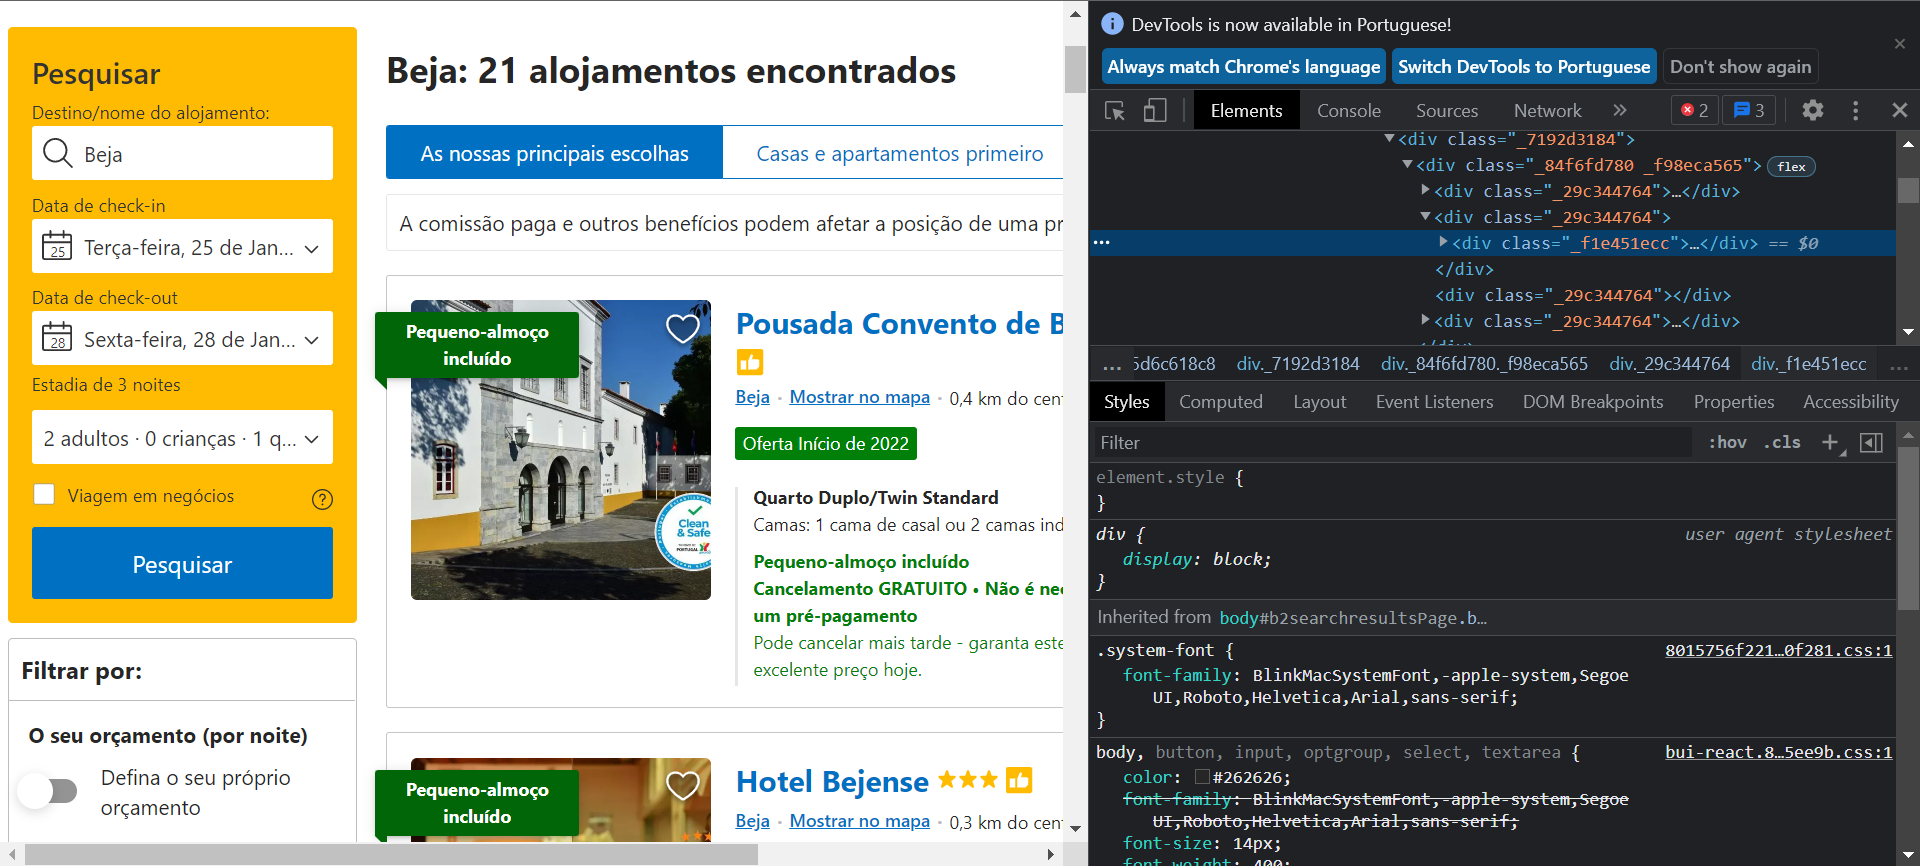
\includegraphics[width=15cm]{booking_com.png}
  \caption{Site Booking.com ao usar a ferramenta inspecionar}
  \label{fig:booking_com}
\end{figure}

\newpage

No código foi implementado as bibliotecas BeautifulSoup para facilitar a tarefa de realizar o ``web-scraping''.

\begin{minted}[linenos,tabsize=2,breaklines,breakanywhere]{python3}
from bs4 import BeautifulSoup
import requests
import pandas as pd
\end{minted}

A partir do ``website'' ao inspeccionar a página era possível retirar os \textit{headers} que eram valores necessários na realização do ``web-scrapping''.
Também é realizado o pedido HTTP e juntou-se a informação com a biblioteca ``BeautifulSoup''.

\begin{minted}[linenos,tabsize=2,breaklines,breakanywhere]{python3}
headers = {
  'User-Agent': 'Mozilla/5.0 (Windows NT 10.0; Win64; x64) AppleWebKit...'}
url = "https://www.booking.com/searchresults.pt-pt.html?..."
response = requests.get(url, headers=headers)
soup = BeautifulSoup(response.content, 'lxml')
\end{minted}

Foram criados diferentes \textit{arrays} para receber as informações e posteriormente colocada a respectiva informação em cada um deles.

\begin{minted}[linenos,tabsize=2,breaklines,breakanywhere]{python3}
hotel = []
badge = []
title = []
reviews = []
price = []
for item in soup.select('.fb3c4512b4'):
    try:
        hotel.append(item.select('.fde444d7ef')[0].get_text().strip())
        badge.append(item.select('._9c5f726ff')[0].get_text().strip())
        title.append(item.select('._192b3a196')[0].get_text().strip())
        reviews.append(item.select('._1e6021d2f')[0].get_text().strip())
        price.append(item.select('._e885fdc12')[0].get_text().strip())
    except Exception as e:
        print('')
\end{minted}

Devido a alguns ``arrays'' conterem mais informação, possivelmente devido a algum tipo de informação adicional que possa estar em algum hotel especificamente, para prevenir erros, foram reduzidos ao tamanho do \textit{array} mais curto.

Por fim todos os resultados contidos nos ``arrays'' foram guardados num ficheiro \text{.csv} denominado ``listtable\text{.csv}''.

\begin{minted}[linenos,tabsize=2,breaklines,breakanywhere]{python3}
d1 = {'Hotel': hotel[:length], 'Classificacao': badge[:length],
    'Suma': title[:length], 'Avaliacoes': reviews[:length], 'Preco': price[:length]}
df = pd.DataFrame.from_dict(d1)
print(df)
df.to_csv('listtable\text{.csv}')
\end{minted}

Construção dos links para realizar o ``web-scraping'' das ``reviews'' de cada hotel.

\begin{minted}[linenos,tabsize=2,breaklines,breakanywhere]{python3}
reviews_links = []
for link in soup.findAll('a', {'class': 'fb01724e5b'}):
    a = link['href']
    hotel = a.split('/')[5].split('?')[0]
    a = 'https://www.booking.com/reviews/pt/hotel/' + hotel
    reviews_links.append(a)
\end{minted}

\newpage

Foi realizado o pedido ``HTTP'' e juntado á biblioteca ``BeautifulSoup'' para aceder ás ``reviews'' de cada site e todos os valores foram salvos no formato \text{.csv}.

\begin{minted}[linenos,tabsize=2,breaklines,breakanywhere]{python3}
count = 0
allreviews = []
for link in reviews_links:
    try:
        response2 = requests.get(link, headers=headers)
        soup2 = BeautifulSoup(response2.content, 'lxml')
        for r in soup2.findAll('span', {'itemprop': 'reviewBody'}):
            try:
                rev = r.text
                allreviews.append(rev + '\n')
            except:
                pass
    except:
        pass
    count += 1
    if allreviews != []:
        seen = set()
        allreviews = [item for item in allreviews if not(
            tuple(item) in seen or seen.add(tuple(item)))]
        dfr = pd.DataFrame.from_dict({'Avaliacoes': allreviews})
        print(dfr)
        dfr.to_csv('hotel' + str(count) + '\text{.csv}')
        allreviews = []
\end{minted}

No final, temos esta tabela representativa do hotéis \textit{scraped} ordenada e representativa dos \textit{scrapes} ``hotelXX.csv''.

\begin{table}[!ht]
  \centering
  \begin{tabular}{|l|l|l|l|}
    \hline
    ~  & Hotel                                              & Classificação & Preço \\ \hline
    0  & Hotel Bejense                                      & ``8,4''       & 189   \\ \hline
    1  & Aljana Guest House Beja                            & ``9,3''       & 330   \\ \hline
    2  & BejaParque Hotel                                   & ``8,1''       & 255   \\ \hline
    3  & Pousada Convento de Beja                           & ``8,7''       & 270   \\ \hline
    4  & Guest House Stories                                & ``8,7''       & 135   \\ \hline
    5  & Hotel Melius                                       & ``8,1''       & 242   \\ \hline
    6  & Casa do Arco - Beja                                & ``9,4''       & 210   \\ \hline
    7  & Barrote Beja- Alojamento Local                     & ``9,7''       & 255   \\ \hline
    8  & Maria`s Guesthouse                                 & ``9,4''       & 226   \\ \hline
    9  & Beja Garden                                        & ``8,0''       & 90    \\ \hline
    10 & HI Beja - Pousada de Juventude                     & ``9,6''       & 327   \\ \hline
    11 & Casa do Sembrano                                   & ``9,5''       & 330   \\ \hline
    12 & Casa Idalina Villa in Beja's beautiful countryside & ``9,4''       & 210   \\ \hline
    13 & Império Romano Guest House                         & ``9,0''       & 150   \\ \hline
    14 & Monte das Beatas - Alojamento Local                & ``8,7''       & 306   \\ \hline
    15 & Casa do Jardim                                     & ``8,8''       & 270   \\ \hline
    16 & Casa das Histórias                                 & ``8,9''       & 195   \\ \hline
    17 & Casa Centro Histórico Beja - Castelo               & ``7,9''       & 180   \\ \hline
    18 & Quinta do Castelo                                  & ``9,0''       & 214   \\ \hline
    19 & Casa do Avô Zé                                     & ``8,1''       & 174   \\ \hline
    20 & Suite na Praça da República                        & ``8,7''       & 228   \\ \hline
    21 & Herdade da Diabroria - Agroturismo                 & ``8,8''       & 285   \\ \hline
    22 & Herdade do Vau                                     & ``7,8''       & 270   \\ \hline
    23 & Monte da Corte Ligeira                             & ``8,3''       & 150   \\ \hline
  \end{tabular}
  \caption{Tabela com todos os hotéis de Beja retirados do Booking.com}
\end{table}

\subsection{Resultados}

Aqui exemplifica-se um ficheiro \text{.csv}, ``hotel18.csv'', que contem os \textit{reviews} do hotel ``Quinta do Castelo''.

\begin{table}[!ht]
  \centering
  \begin{adjustbox}{width=\columnwidth,center}
    \begin{tabular}{|l|l|}
      \hline
      ~     & Opiniões                                                                                                                                     \\ \hline
      0     & A localização é excelente assim como as condições do espaço. Local muito bem cuidado e apelativo. Fomos muito bem recebidos \dots            \\ \hline
      1     & Nada digno de registo.                                                                                                                       \\ \hline
      2     & A simpatia da Sra Catarina foi fantástica. A casa e as acomodações corresponderam ás expetivas e relação qualidade preço foi perfeita \ldots \\ \hline
      3     & Localização excelente, apartamento espaçoso, e totalmente equipado.
      O facto de ser uma construção antiga, cria um ambiente muito \ldots                                                                                  \\ \hline
      4     & A localização é impecável mesmo no centro histórico de Beja. Casa Limpa e organizada. Dona super prestável e e simpática.                    \\ \hline
      5     & De noite ouve-se o barulho da rua com muita facilidade.                                                                                      \\ \hline
      6     & A casa está muito perto do castelo e está muito bem decorada e limpa. Muito agradável!                                                       \\ \hline
      7     & O dono não tem culpa mas a zona não é muito bem frequentada á noite                                                                          \\ \hline
      8     & A casa é muito gira e funcional!                                                                                                             \\ \hline
      9     & Casa muito agradável e bem situada.  Os anfitriães são simpáticos e disponíveis. Cozinha muito bem equipada e casa de banho excelente.       \\ \hline
      10    & Da localização, da relação preço/qualidade que entendo adequada.                                                                             \\ \hline
      11    & Localização no centro histórico tem vantagens (centralidade) e desvantagens (dificuldades de estacionamento).                                \\ \hline
      12    & Localização, decoração, conforto, organização do espaço e o gosto cuidado na decoração.                                                      \\ \hline
      13    & Não tinha microondas.                                                                                                                        \\ \hline
      14    & Localização, estacionamento perto, a decoração do alojamento, ter máquina de lavar roupa deu muito geito.                                    \\ \hline
      15    & Virado para duas ruas públicas isso condiciona a entrada de luz e de ventilação em casa pela noção de segurança;
      Existem algumas \ldots
      \\ \hline
      16    & A casa em si é antiga e possui algumas divisões de formatos, alturas, níveis de pavimento e arcadas distintas, o que lhe dão um ar \ldots
      \\ \hline
      17    & Poderia ter um microondas.                                                                                                                   \\ \hline
      18    & Muito bem localizado, anfitriões muito simpáticos.
      Muito interessante a manutenção de casa típica alentejana.
      Gostamos todos muito \ldots
      \\ \hline
      19    & Gostei de tudo. Não tenho do q reclamar.                                                                                                    \\ \hline
      20    & O apartamento é uma graça. Super completo, amplo, decorado com muito bom gosto e jovial! Adorei!!!!!                                         \\ \hline
      21    & Serviço conforto e localização.                                                                                                              \\ \hline
      22    & A limpeza poderia ser mais cuidada. Não dar para ligar a chaleira eléctrica porque o quadro não aguentava. O fogão estar rachado \ldots      \\ \hline
      23    & Da receção, da decoração, da temperatura da casa, o ser uma casa acolhedora situada no coração do centro histórico.                          \\ \hline
      \dots & \dots                                                                                                                                        \\ \hline
      28    & De tudo. Um lugar ótimo para uma família passar uns dias, a casa está bem situada e as pessoas muito simpáticas. Um lugar a repetir.         \\ \hline
    \end{tabular}
  \end{adjustbox}
  \caption{Tabela de resultados de algumas ``Reviews'' para um dos hotéis (hotel18\text{.csv})}
\end{table}

\newpage

\section{Zomato}

A Zomato é um serviço de busca de restaurantes para quem quer sair para jantar, buscar comida ou pedir em casa. A Zomato possui duas secções: guia de restaurante e blog. Previamente, havia uma secção de eventos, já descontinuada.

O guia de restaurantes Zomato permite ao usuário buscar informações relacionadas a restaurantes, bares, cafés, pubs e casa nocturnas. As informações fornecidas geralmente incluem o nome do estabelecimento, telefones de contacto, endereço, cardápio, fotografias, avaliações e mapas de localização.

\subsection{Estratégia}

As páginas da \textit{web app} do Zomato usam um ``paralax'' de \textit{scrolling} infinito (até não haver mais restaurantes) e as classes dos ``HTML tags'' mudam por sessão e/ou \textit{rendering}, logo aqui a estratégia é literalmente fazer ``download'' da página web e fazer o \textit{scrape} a partir do \textit{parsing} dessa página.

\subsection{Desenvolvimento}

Aqui é representada uma aproximação do desenvolvimento deste \textit{scraping}.

\subsubsection{Restaurantes}

Primeiramente foi feito o \textit{import} das bibliotecas.

\begin{minted}[linenos,tabsize=2,breaklines,breakanywhere]{python3}
from bs4 import BeautifulSoup
import requests
import pandas as pd
\end{minted}

Depois pegando no código dos colegas como \textit{template}, adaptou-se para usar uma página previamente descarregada.

\begin{minted}[linenos,tabsize=2,breaklines,breakanywhere]{python3}
headers = {
   "User-Agent": "Mozilla/5.0 (Linux; Android 6.0; Nexus 5 Build/MRA58N) AppleWebKit/537.36 (KHTML, like Gecko) Chrome/96.0.4664.93 Mobile Safari/537.36",
}
soup = BeautifulSoup(open(r"C:\Users\vitor\Desktop\pi2021\projecto\webscrape\scrapes\zomato\restaurantes\zomato-beja-14-dez.html", encoding="utf8").read(), 'lxml')
\end{minted}

Fazemos um ciclo de \textit{scraping} dos nomes dos locais de consumo.

\begin{minted}[linenos,tabsize=2,breaklines,breakanywhere]{python3}
restaurant = []
for name in soup.findAll('h4',{'class':'sc-1hp8d8a-0'}):
    restaurant.append(name.text.strip())
print(len(restaurant))
\end{minted}

E agora dois ciclos, um para as classes com nome gerado no \textit{prerender} e outra pós \textit{render}; vamos buscar os tipos/classes de restaurantes.

\begin{minted}[linenos,tabsize=2,breaklines,breakanywhere]{python3}
type = []
for name in soup.findAll('p',{'class':'jaKOQh'}):
    print(name)
    type.append(name.text.strip())
for name in soup.findAll('p',{'class':'kegdaG'}):
    print(name)
    type.append(name.text.strip())
print(len(type))
\end{minted}

E outros dois ciclos do mesmo motivo, para ir buscar os preços.

\begin{minted}[linenos,tabsize=2,breaklines,breakanywhere]{python3}
price = []
for p in soup.findAll('p',{'class':'ftdqla'}):
  price.append(p.text.replace('euros para dois','').strip())
for p in soup.findAll('p',{'class':'kOONhy'}):
  price.append(p.text.replace('euros para dois','').strip())
print(len(price))
\end{minted}

Com o código seguinte geramos um \textit{dataframe} que exporta um \text{.csv}.

\begin{minted}[linenos,tabsize=2,breaklines,breakanywhere]{python3}
d1 = {'Restaurante': restaurant[:length],'Tipo':type[:length],'Preco':price[:length]}
df = pd.DataFrame.from_dict(d1)
print(df)
df.to_csv('listtable.csv')
\end{minted}

Que gerou um ficheiro aqui representado nesta tabela:

\begin{table}[!ht]
  \centering
  \begin{tabular}{|l|l|l|l|}
    \hline
    ~      & Restaurante                 & Tipo                                & Preço  \\ \hline
    0      & Adega Típica 25 de Abril    & Alentejana, Portuguesa              & 25     \\ \hline
    1      & Dom Dinis                   & Bifes, Portuguesa                   & 30     \\ \hline
    2      & Sushi Alentejano            & Sushi, Japonesa                     & 35     \\ \hline
    3      & Herdade dos Grous           & Contemporânea, Portuguesa           & 60     \\ \hline
    4      & Pulo do Lobo                & Portuguesa                          & 25     \\ \hline
    5      & Bar Parque da Vila Beringel & Snacks, Bebidas                     & 12     \\ \hline
    6      & Figa's                      & Pizza, Italiana                     & 25     \\ \hline
    7      & Cervejaria Portugalo        & Portuguesa, Bebidas, Petiscos       & 25     \\ \hline
    8      & Entre Arcos                 & Portuguesa, Grelhados               & 25     \\ \hline
    9      & Aperitivo                   & Bebidas, Portuguesa                 & 20     \\ \hline
    10     & O Arbitro                   & Portuguesa                          & 25     \\ \hline
    11     & Café Central                & Snacks, Bebidas, Portuguesa         & 15     \\ \hline
    12     & Gatus Cervejaria Alentejana & Alentejana, Portuguesa, Marisqueira & 25     \\ \hline
    13     & Hamburgueria da Avenida     & Hamburgueria                        & 25     \\ \hline
    14     & Casa de Pasto O Forno       & Snacks, Bebidas, Portuguesa         & 12     \\ \hline
    15     & Tennis Courts Club          & Portuguesa                          & 25     \\ \hline
    16     & Cervejaria Mira Serra       & Marisqueira, Portuguesa             & 40     \\ \hline
    17     & Espelho d'Água              & Portuguesa                          & 25     \\ \hline
    18     & TEM Avondo                  & Portuguesa, Alentejana              & 25     \\ \hline
    19     & Menau                       & rtuguesa                            & 25     \\ \hline
    20     & Toy Faróis                  & Portuguesa, Grelhados               & 25     \\ \hline
    21     & Taberna A Pipa              & Alentejana, Portuguesa, Petiscos    & 25     \\ \hline
    22     & Pizzeria Milano             & Pizza, Italiana, Portuguesa         & 25     \\ \hline
    23     & Dona Maria Deck             & Portuguesa, Petiscos, Snacks        & 25     \\ \hline
    24     & O Alemão                    & Portuguesa, Petiscos, Alentejana    & 25     \\ \hline
    25     & Deliciosa Alvorada          & Portuguesa, Alentejana              & 25     \\ \hline
    26     & Moments IPDJ                & Portuguesa                          & 20     \\ \hline
    27     & Bar Regional                & Bebidas, Snacks                     & 6      \\ \hline
    28     & Sushizzaria                 & Sushi, Hamburgueria, Pizza          & 30     \\ \hline
    \ldots & \ldots                      & \ldots                              & \ldots \\ \hline
    155    & Vegetariano                 & Vegetariana                         & 25     \\ \hline
  \end{tabular}
  \caption{Tabela dos restaurantes}
\end{table}

\newpage

Agora, pelo mesmo motivo, dois ciclos; que vão buscar os links das páginas dos \textit{reviews}.

\begin{minted}[linenos,tabsize=2,breaklines,breakanywhere]{python3}
reviews_links = []
for link in soup.findAll('a', {'class': 'ieKty'}):
    a = link['href']
    reviews_links.append(a.replace('/info', '/reviews'))
for link in soup.findAll('a', {'class': 'jjSAcU'}):
    a = link['href']
    reviews_links.append(a.replace('/info', '/reviews'))
\end{minted}

O qual extraímos todos os ``tags'' de parágrafos porque que sempre que se corria o código gerava uma classe nova\ldots Logo, estas extracções desapontantes, vão sofrer ETL.

\begin{minted}[linenos,tabsize=2,breaklines,breakanywhere]{python3}
count = 0
allreviews = []
for link in reviews_links:
    try:
        response2 = requests.get(link, headers=headers)
        soup2 = BeautifulSoup(response2.content, 'lxml')
        for r in soup2.findAll('p'): # sempre a mudar a class, vai sofrer ETL
            try:
                rev = r.text
                # print(rev)
                allreviews.append(rev + '\n')
            except:
                pass
    except:
        pass
    count += 1
    if allreviews != []:
        seen = set()
        allreviews = [item for item in allreviews if not(
            tuple(item) in seen or seen.add(tuple(item)))]
        dfr = pd.DataFrame.from_dict({'Avaliacoes': allreviews})
        print(dfr)
        dfr.to_csv('restaurante' + str(count) + '.csv')
        allreviews = []
\end{minted}

\subsection{Resultados}

Os resultados deste \textit{scrape} foram desapontantes no minimo devido à infeliz \textit{random generated} nome da classe, que é gerado por cada vez que se usa a página. Estes resultados vão sofrer muito ETL posterior.

\begin{table}[!ht]
  \centering
  \begin{adjustbox}{width=\columnwidth,center}
    \begin{tabular}{|l|l|}
      \hline
      ~      & Avaliações                                                                                           \\ \hline
      \ldots & \ldots                                                                                               \\ \hline
      5      & "Matilde Almeida"                                                                                    \\ \hline
      6      & "Há 4 meses"                                                                                         \\ \hline
      7      & "Um restaurante de excelente qualidade. A deliciosa comida típica de Beja e muito bem servida\ldots" \\ \hline
      8      & "0 Votes for helpful, 0 Comentários"                                                                 \\ \hline
      9      & "CláudiaSimões"                                                                                      \\ \hline
      10     & "Há 6 meses"                                                                                         \\ \hline
      11     & "Desde que venho passar férias a Beja que comecei a vir a este restaurante\ldots"                    \\ \hline
      \ldots & \ldots                                                                                               \\ \hline
    \end{tabular}
  \end{adjustbox}
  \caption{Tabela de resultados do ``restaurante1.csv''}
\end{table}

\newpage

\section{Próximos Passos}

Na seguinte fase de trabalho o grupo irá ter que começar a desenvolver os métodos dos quais criaremos um modelo de \textit{machine learning} para analise de sentimento e extracção de tópicos e \textit{keywords} para associar \textit{reviews} e \textit{listings}.

Para tal é necessário previamente usar processos de ETL \textit{(extract, transform, load)} do trabalho já realizado, uma das tarefas será a adaptação de todo o conteúdo textual já armazenado e reparação de informação corrupta e remoção de informação.

\section{Conclusão}

Concluindo, este trabalho, de forma análoga e pessoal, serviu para aprender o que realmente é o ``web-scraping'' e todos os usos que ele pode ter para a recolha de dados estruturados da web; já da forma curricular, serviu do primeiro passo, de acesso à informação necessária para a analise sentimental e textual sobre o turismo rural sul-alentejano.

Para além de aprender o que ele realmente é, também tivemos a oportunidade de trabalhar com ele e usá-lo num caso prático.

Houveram algumas dúvidas principalmente para retirar algumas informações de alguns dos ``websites'' trabalhados e também na criação do ambiente virtual, porem todas as duvidas foram superadas graças ao trabalho em equipa e pesquisas online, para alem da ajuda da docente responsável pelo projecto.

Por fim, achamos que o balanço desta parte do trabalho tenha sido bastante positiva.

\section{Webgrafia}

\renewcommand{\bibsection}{}
\bibliography{webscraping.bib}

\end{document}
